\documentclass{article}

\usepackage{graphicx}
\usepackage{tikz}
\usepackage{tikzsymbols}
\usetikzlibrary{calc,patterns,shapes.geometric}
\pagestyle{empty}
\usepackage[margin=0pt]{geometry}
\geometry{papersize={14in,12in}}

\def\centerarc[#1](#2)(#3:#4:#5){\draw[#1] ($(#2)+({#5*cos(#3)},{#5*sin(#3)})$) arc (#3:#4:#5);}

\begin{document}
	\begin{figure}
		\centering
		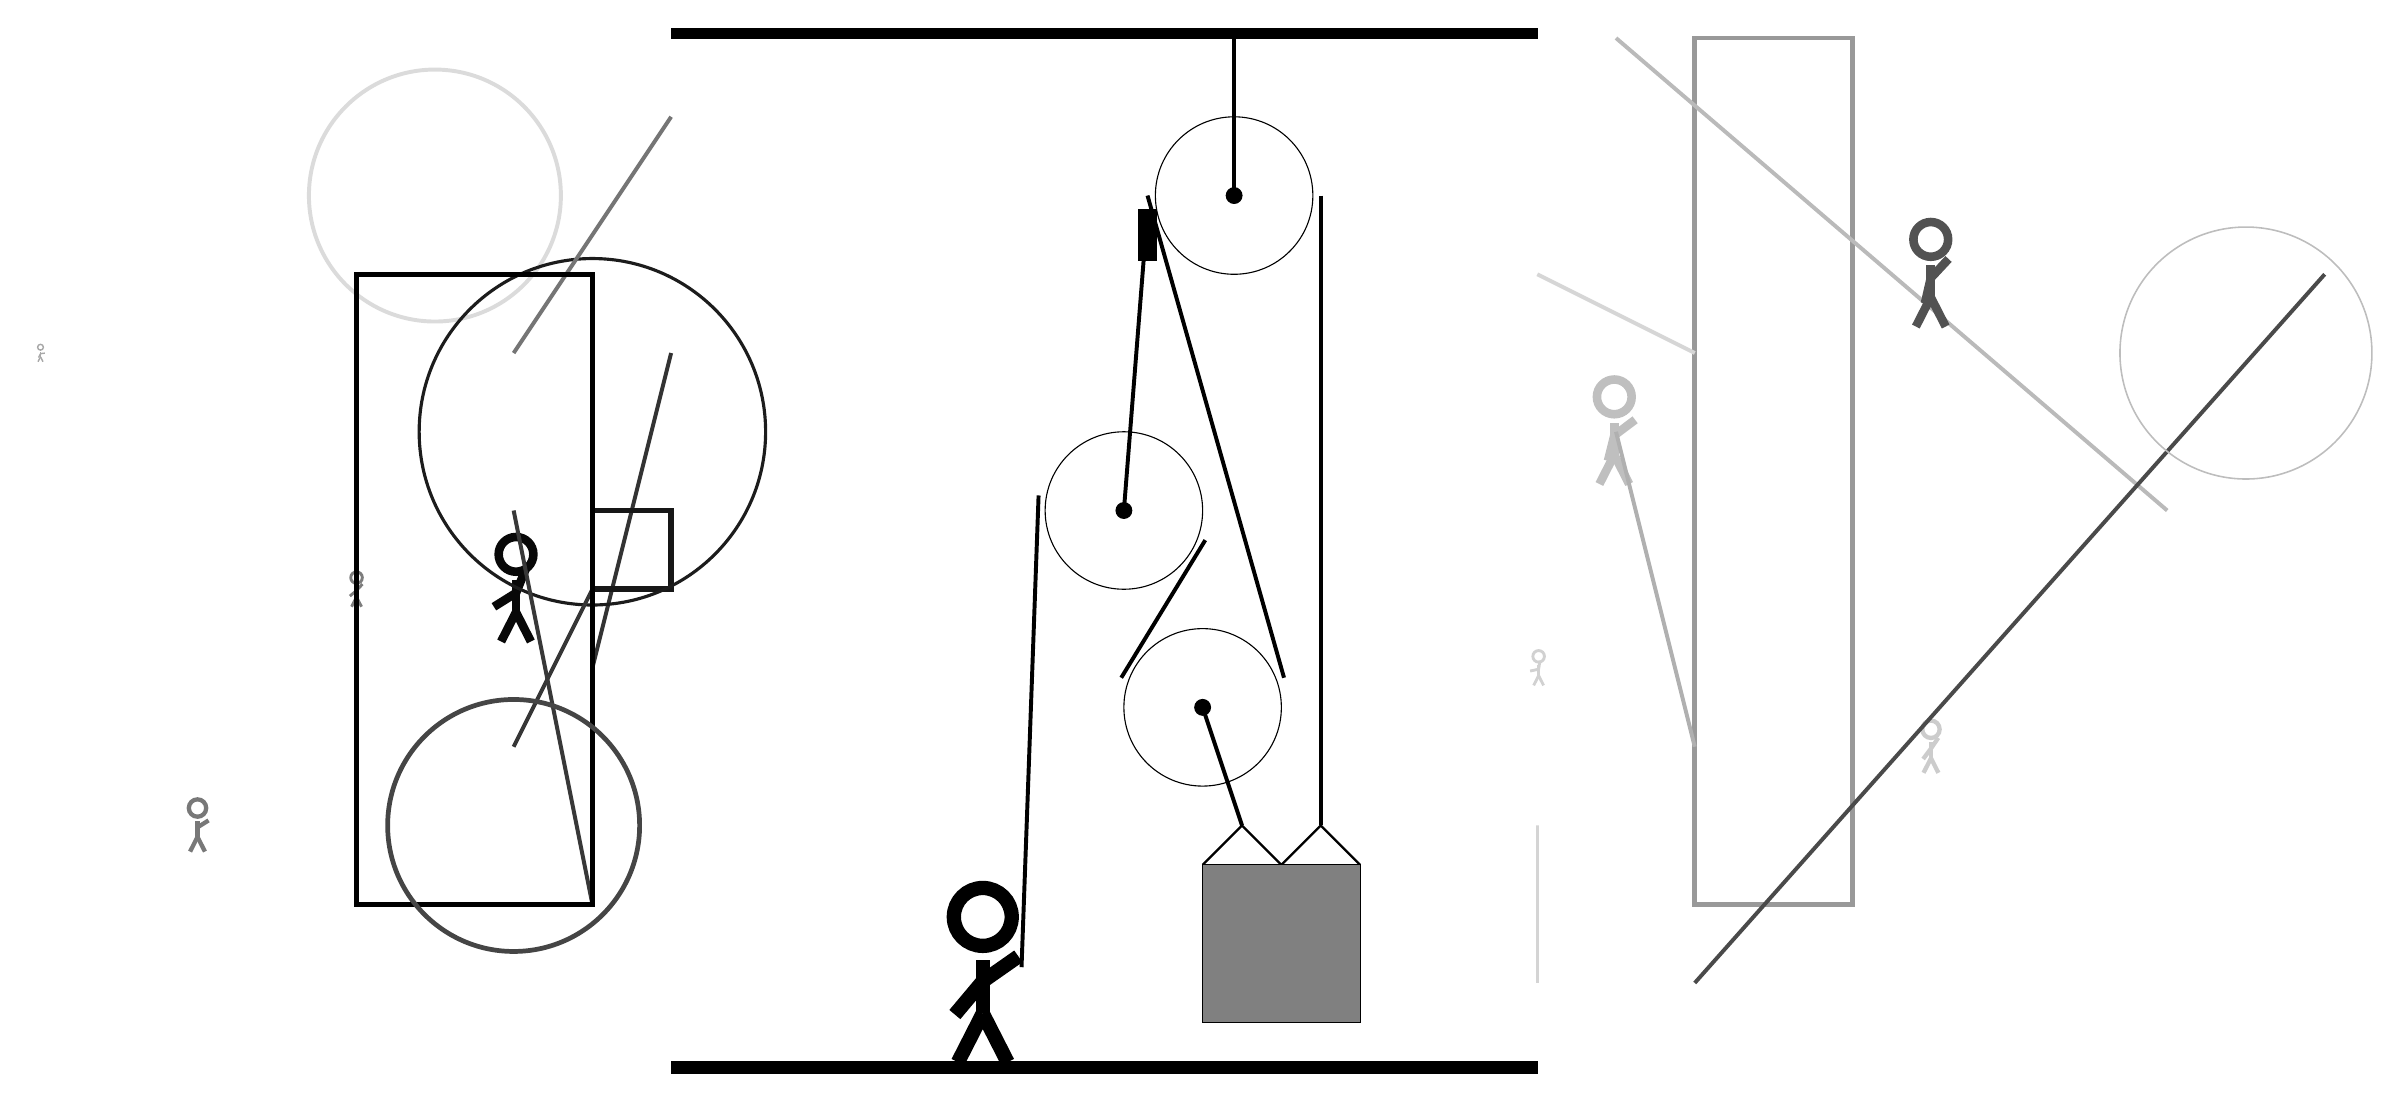
\begin{tikzpicture}
			%%%%% START %%%%%
			
			\draw[fill=black] (-6, 10) rectangle (5, 10.125);
			
			\draw (-0.25, 4.0) circle (1);
			\draw[fill=black] (-0.25, 4.0) circle (0.1);
			
			\draw (0.75, 1.5) circle (1);
			\draw[fill=black] (0.75, 1.5) circle (0.1);
			
			\draw (1.15, 8.0) circle (1);
			\draw[fill=black] (1.15, 8.0) circle (0.1);
			\draw[very thick] (1.15, 8.0) -- (1.15, 10);
			
			\draw[line width=0.5mm, color=black!80](-6, 6) -- (-7, 2);
			
			\node[line width=0.4mm, color=black!25] at (6, 5) {\Strichmaxerl[6][76][37]};
			\draw[line width=0.6mm, color=black!40] (7, -1) rectangle (9, 10);
			\draw[line width=0.5mm, color=black!31](6, 5) -- (7, 1);
			
			\draw [line width=0.5mm, color=black!14](-9, 8) circle (1.6);
			\node[line width=0.5mm, color=black!18] at (5, 2) {\Strichmaxerl[2][12][81]};
			\node[line width=0.5mm, color=black!97] at (-8, 3) {\Strichmaxerl[6][32][68]};
			\draw[line width=0.7mm, color=black!91] (-6, 3) rectangle (-7, 4);
			\draw [line width=0.4mm, color=black!89](-7, 5) circle (2.2);
			
			\node[line width=0.6mm, color=black!20] at (10, 1) {\Strichmaxerl[3][53][56]};
			\draw[line width=0.5mm, color=black!27](6, 10) -- (13, 4);
			
			\draw[line width=0.5mm, color=black!54](-8, 6) -- (-6, 9);
			\draw[line width=0.5mm, color=black!79](-8, 1) -- (-7, 3);
			
			\node[line width=0.3mm, color=black!68] at (10, 7) {\Strichmaxerl[6][77][47]};
			\draw[line width=0.5mm, color=black!78](-7, -1) -- (-8, 4);
			\node[line width=0.5mm, color=black!53] at (-12, 0) {\Strichmaxerl[3][89][32]};
			
			\node[line width=0.3mm, color=black!34] at (-14, 6) {\Strichmaxerl[1][63][7]};
			\draw[line width=0.5mm, color=black!16](5, 7) -- (7, 6);
			\draw[line width=0.5mm, color=black!71](7, -2) -- (15, 7);
			
			\draw [line width=0.2mm, color=black!26](14, 6) circle (1.6);
			\node[line width=0.6mm, color=black!51] at (-10, 3) {\Strichmaxerl[2][40][47]};
			\draw[line width=0.6mm, color=black!100] (-7, 7) rectangle (-10, -1);
			\draw[line width=0.4mm, color=black!17] (5, 0) rectangle (5, -2);
			\draw [line width=0.6mm, color=black!73](-8, 0) circle (1.6);
			
			\draw[thick]  (0.75, -0.5) -- (1.25, 0.0) -- (1.75, -0.5) -- (2.25, 0.0) -- (2.75, -0.5);
			\draw[fill=black!50] (0.75, -0.5) rectangle (2.75, -2.5);
			
			\draw[line width=0.5mm] (-0.25, 4.0) -- (0.05, 7.8);
			\draw[line width=0.5mm, fill=black](-0.05, 7.2) rectangle (0.15, 7.8);
			\draw[line width=0.5mm] (-1.55, -1.8) -- (-1.3333, 4.191);
			\centerarc[line width=0.5mm](-0.25, 4.0)(-20:170:1.1);
			\draw[line width=0.5mm] (0.7837, 3.6238) -- (-0.2837, 1.8762);
			\centerarc[line width=0.5mm](0.75, 1.5)(160:380:1.1);
			\draw[line width=0.5mm] (1.7837, 1.8762) -- (0.05, 8.0);
			\draw[line width=0.5mm](0.75, 1.5) -- (1.25, 0.0);
			\centerarc[line width=0.5mm](1.15, 8.0)(0:180:1.1);
			\draw[line width=0.5mm] (2.25, 8.0) -- (2.25, 0.0);
			
			\node at (-2, -1.9) {\Strichmaxerl[10][50][35]};
			
			\draw[fill=black] (-6, -3) rectangle (5, -3.15);
			
			%%%%% END %%%%%
		\end{tikzpicture}
	\end{figure}	
\end{document}